\documentclass[twoside]{book}

% Packages required by doxygen
\usepackage{fixltx2e}
\usepackage{calc}
\usepackage{doxygen}
\usepackage[export]{adjustbox} % also loads graphicx
\usepackage{graphicx}
\usepackage[utf8]{inputenc}
\usepackage{makeidx}
\usepackage{multicol}
\usepackage{multirow}
\PassOptionsToPackage{warn}{textcomp}
\usepackage{textcomp}
\usepackage[nointegrals]{wasysym}
\usepackage[table]{xcolor}

% Font selection
\usepackage[T1]{fontenc}
\usepackage[scaled=.90]{helvet}
\usepackage{courier}
\usepackage{amssymb}
\usepackage{sectsty}
\renewcommand{\familydefault}{\sfdefault}
\allsectionsfont{%
  \fontseries{bc}\selectfont%
  \color{darkgray}%
}
\renewcommand{\DoxyLabelFont}{%
  \fontseries{bc}\selectfont%
  \color{darkgray}%
}
\newcommand{\+}{\discretionary{\mbox{\scriptsize$\hookleftarrow$}}{}{}}

% Page & text layout
\usepackage{geometry}
\geometry{%
  a4paper,%
  top=2.5cm,%
  bottom=2.5cm,%
  left=2.5cm,%
  right=2.5cm%
}
\tolerance=750
\hfuzz=15pt
\hbadness=750
\setlength{\emergencystretch}{15pt}
\setlength{\parindent}{0cm}
\setlength{\parskip}{3ex plus 2ex minus 2ex}
\makeatletter
\renewcommand{\paragraph}{%
  \@startsection{paragraph}{4}{0ex}{-1.0ex}{1.0ex}{%
    \normalfont\normalsize\bfseries\SS@parafont%
  }%
}
\renewcommand{\subparagraph}{%
  \@startsection{subparagraph}{5}{0ex}{-1.0ex}{1.0ex}{%
    \normalfont\normalsize\bfseries\SS@subparafont%
  }%
}
\makeatother

% Headers & footers
\usepackage{fancyhdr}
\pagestyle{fancyplain}
\fancyhead[LE]{\fancyplain{}{\bfseries\thepage}}
\fancyhead[CE]{\fancyplain{}{}}
\fancyhead[RE]{\fancyplain{}{\bfseries\leftmark}}
\fancyhead[LO]{\fancyplain{}{\bfseries\rightmark}}
\fancyhead[CO]{\fancyplain{}{}}
\fancyhead[RO]{\fancyplain{}{\bfseries\thepage}}
\fancyfoot[LE]{\fancyplain{}{}}
\fancyfoot[CE]{\fancyplain{}{}}
\fancyfoot[RE]{\fancyplain{}{\bfseries\scriptsize Generated by Doxygen }}
\fancyfoot[LO]{\fancyplain{}{\bfseries\scriptsize Generated by Doxygen }}
\fancyfoot[CO]{\fancyplain{}{}}
\fancyfoot[RO]{\fancyplain{}{}}
\renewcommand{\footrulewidth}{0.4pt}
\renewcommand{\chaptermark}[1]{%
  \markboth{#1}{}%
}
\renewcommand{\sectionmark}[1]{%
  \markright{\thesection\ #1}%
}

% Indices & bibliography
\usepackage{natbib}
\usepackage[titles]{tocloft}
\setcounter{tocdepth}{3}
\setcounter{secnumdepth}{5}
\makeindex

% Hyperlinks (required, but should be loaded last)
\usepackage{ifpdf}
\ifpdf
  \usepackage[pdftex,pagebackref=true]{hyperref}
\else
  \usepackage[ps2pdf,pagebackref=true]{hyperref}
\fi
\hypersetup{%
  colorlinks=true,%
  linkcolor=blue,%
  citecolor=blue,%
  unicode%
}

% Custom commands
\newcommand{\clearemptydoublepage}{%
  \newpage{\pagestyle{empty}\cleardoublepage}%
}

\usepackage{caption}
\captionsetup{labelsep=space,justification=centering,font={bf},singlelinecheck=off,skip=4pt,position=top}

%===== C O N T E N T S =====

\begin{document}

% Titlepage & ToC
\hypersetup{pageanchor=false,
             bookmarksnumbered=true,
             pdfencoding=unicode
            }
\pagenumbering{roman}
\begin{titlepage}
\vspace*{7cm}
\begin{center}%
{\Large My Project }\\
\vspace*{1cm}
{\large Generated by Doxygen 1.8.11}\\
\end{center}
\end{titlepage}
\clearemptydoublepage
\tableofcontents
\clearemptydoublepage
\pagenumbering{arabic}
\hypersetup{pageanchor=true}

%--- Begin generated contents ---
\chapter{Class Index}
\section{Class List}
Here are the classes, structs, unions and interfaces with brief descriptions\+:\begin{DoxyCompactList}
\item\contentsline{section}{\hyperlink{structnode}{node} }{\pageref{structnode}}{}
\item\contentsline{section}{\hyperlink{structnode1}{node1} }{\pageref{structnode1}}{}
\item\contentsline{section}{\hyperlink{structnode__info}{node\+\_\+info} }{\pageref{structnode__info}}{}
\end{DoxyCompactList}

\chapter{File Index}
\section{File List}
Here is a list of all files with brief descriptions\+:\begin{DoxyCompactList}
\item\contentsline{section}{\hyperlink{Lab1_8c}{Lab1.\+c} }{\pageref{Lab1_8c}}{}
\end{DoxyCompactList}

\chapter{Class Documentation}
\hypertarget{classstudent}{}\section{student Class Reference}
\label{classstudent}\index{student@{student}}
\subsection*{Public Member Functions}
\begin{DoxyCompactItemize}
\item 
void \hyperlink{classstudent_a9516948671b936201a0daac50ad4ca6f}{get\+Details} (void)
\item 
void \hyperlink{classstudent_a2de761d21703bd2b530de4cbc5eed372}{put\+Details} (void)
\end{DoxyCompactItemize}
\subsection*{Private Attributes}
\begin{DoxyCompactItemize}
\item 
char \hyperlink{classstudent_a87db2e64ee10a8c37a9c2657c5da5228}{name} \mbox{[}30\mbox{]}
\item 
int \hyperlink{classstudent_aba65fad741cdd2d47b62592e0a02aa05}{roll\+No}
\item 
int \hyperlink{classstudent_a036cbac5ccbb235fdc3313cb7806e199}{total}
\item 
float \hyperlink{classstudent_a63ba5c58c9d2bfe2c7f3128eb0222637}{perc}
\end{DoxyCompactItemize}


\subsection{Member Function Documentation}
\index{student@{student}!get\+Details@{get\+Details}}
\index{get\+Details@{get\+Details}!student@{student}}
\subsubsection[{\texorpdfstring{get\+Details(void)}{getDetails(void)}}]{\setlength{\rightskip}{0pt plus 5cm}void student\+::get\+Details (
\begin{DoxyParamCaption}
\item[{void}]{}
\end{DoxyParamCaption}
)}\hypertarget{classstudent_a9516948671b936201a0daac50ad4ca6f}{}\label{classstudent_a9516948671b936201a0daac50ad4ca6f}

\begin{DoxyCode}
24                             \{
25     cout << \textcolor{stringliteral}{"Enter name: "} ;
26     cin >> \hyperlink{classstudent_a87db2e64ee10a8c37a9c2657c5da5228}{name};
27     cout << \textcolor{stringliteral}{"Enter roll number: "};
28     cin >> \hyperlink{classstudent_aba65fad741cdd2d47b62592e0a02aa05}{rollNo};
29     cout << \textcolor{stringliteral}{"Enter total marks outof 500: "};
30     cin >> \hyperlink{classstudent_a036cbac5ccbb235fdc3313cb7806e199}{total};
31      
32     \hyperlink{classstudent_a63ba5c58c9d2bfe2c7f3128eb0222637}{perc}=(float)total/500*100;
33 \}
\end{DoxyCode}
\index{student@{student}!put\+Details@{put\+Details}}
\index{put\+Details@{put\+Details}!student@{student}}
\subsubsection[{\texorpdfstring{put\+Details(void)}{putDetails(void)}}]{\setlength{\rightskip}{0pt plus 5cm}void student\+::put\+Details (
\begin{DoxyParamCaption}
\item[{void}]{}
\end{DoxyParamCaption}
)}\hypertarget{classstudent_a2de761d21703bd2b530de4cbc5eed372}{}\label{classstudent_a2de761d21703bd2b530de4cbc5eed372}

\begin{DoxyCode}
36                             \{
37     cout << \textcolor{stringliteral}{"Student details:\(\backslash\)n"};
38     cout << \textcolor{stringliteral}{"Name:"}<< \hyperlink{classstudent_a87db2e64ee10a8c37a9c2657c5da5228}{name} << \textcolor{stringliteral}{",Roll Number:"} << \hyperlink{classstudent_aba65fad741cdd2d47b62592e0a02aa05}{rollNo} << \textcolor{stringliteral}{",Total:"} << 
      \hyperlink{classstudent_a036cbac5ccbb235fdc3313cb7806e199}{total} << \textcolor{stringliteral}{",Percentage:"} << \hyperlink{classstudent_a63ba5c58c9d2bfe2c7f3128eb0222637}{perc};
39 \}
\end{DoxyCode}


\subsection{Member Data Documentation}
\index{student@{student}!name@{name}}
\index{name@{name}!student@{student}}
\subsubsection[{\texorpdfstring{name}{name}}]{\setlength{\rightskip}{0pt plus 5cm}char student\+::name\mbox{[}30\mbox{]}\hspace{0.3cm}{\ttfamily [private]}}\hypertarget{classstudent_a87db2e64ee10a8c37a9c2657c5da5228}{}\label{classstudent_a87db2e64ee10a8c37a9c2657c5da5228}
\index{student@{student}!perc@{perc}}
\index{perc@{perc}!student@{student}}
\subsubsection[{\texorpdfstring{perc}{perc}}]{\setlength{\rightskip}{0pt plus 5cm}float student\+::perc\hspace{0.3cm}{\ttfamily [private]}}\hypertarget{classstudent_a63ba5c58c9d2bfe2c7f3128eb0222637}{}\label{classstudent_a63ba5c58c9d2bfe2c7f3128eb0222637}
\index{student@{student}!roll\+No@{roll\+No}}
\index{roll\+No@{roll\+No}!student@{student}}
\subsubsection[{\texorpdfstring{roll\+No}{rollNo}}]{\setlength{\rightskip}{0pt plus 5cm}int student\+::roll\+No\hspace{0.3cm}{\ttfamily [private]}}\hypertarget{classstudent_aba65fad741cdd2d47b62592e0a02aa05}{}\label{classstudent_aba65fad741cdd2d47b62592e0a02aa05}
\index{student@{student}!total@{total}}
\index{total@{total}!student@{student}}
\subsubsection[{\texorpdfstring{total}{total}}]{\setlength{\rightskip}{0pt plus 5cm}int student\+::total\hspace{0.3cm}{\ttfamily [private]}}\hypertarget{classstudent_a036cbac5ccbb235fdc3313cb7806e199}{}\label{classstudent_a036cbac5ccbb235fdc3313cb7806e199}


The documentation for this class was generated from the following file\+:\begin{DoxyCompactItemize}
\item 
\hyperlink{StudentDetails_8cpp}{Student\+Details.\+cpp}\end{DoxyCompactItemize}

\chapter{File Documentation}
\hypertarget{StudentDetails_8cpp}{}\section{Student\+Details.\+cpp File Reference}
\label{StudentDetails_8cpp}\index{Student\+Details.\+cpp@{Student\+Details.\+cpp}}
{\ttfamily \#include $<$iostream$>$}\\*
Include dependency graph for Student\+Details.\+cpp\+:
\nopagebreak
\begin{figure}[H]
\begin{center}
\leavevmode
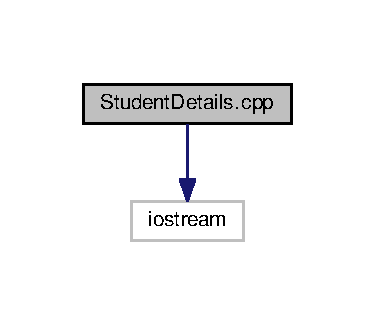
\includegraphics[width=180pt]{StudentDetails_8cpp__incl}
\end{center}
\end{figure}
\subsection*{Classes}
\begin{DoxyCompactItemize}
\item 
class \hyperlink{classstudent}{student}
\end{DoxyCompactItemize}
\subsection*{Macros}
\begin{DoxyCompactItemize}
\item 
\#define \hyperlink{StudentDetails_8cpp_a392fb874e547e582e9c66a08a1f23326}{M\+AX}~10
\end{DoxyCompactItemize}
\subsection*{Functions}
\begin{DoxyCompactItemize}
\item 
int \hyperlink{StudentDetails_8cpp_ae66f6b31b5ad750f1fe042a706a4e3d4}{main} ()
\end{DoxyCompactItemize}


\subsection{Macro Definition Documentation}
\index{Student\+Details.\+cpp@{Student\+Details.\+cpp}!M\+AX@{M\+AX}}
\index{M\+AX@{M\+AX}!Student\+Details.\+cpp@{Student\+Details.\+cpp}}
\subsubsection[{\texorpdfstring{M\+AX}{MAX}}]{\setlength{\rightskip}{0pt plus 5cm}\#define M\+AX~10}\hypertarget{StudentDetails_8cpp_a392fb874e547e582e9c66a08a1f23326}{}\label{StudentDetails_8cpp_a392fb874e547e582e9c66a08a1f23326}


\subsection{Function Documentation}
\index{Student\+Details.\+cpp@{Student\+Details.\+cpp}!main@{main}}
\index{main@{main}!Student\+Details.\+cpp@{Student\+Details.\+cpp}}
\subsubsection[{\texorpdfstring{main()}{main()}}]{\setlength{\rightskip}{0pt plus 5cm}int main (
\begin{DoxyParamCaption}
{}
\end{DoxyParamCaption}
)}\hypertarget{StudentDetails_8cpp_ae66f6b31b5ad750f1fe042a706a4e3d4}{}\label{StudentDetails_8cpp_ae66f6b31b5ad750f1fe042a706a4e3d4}

\begin{DoxyCode}
42 \{
43     \hyperlink{classstudent}{student} \hyperlink{namespacestd}{std}[\hyperlink{StudentDetails_8cpp_a392fb874e547e582e9c66a08a1f23326}{MAX}];       \textcolor{comment}{//array of objects creation}
44     \textcolor{keywordtype}{int} n,loop;
45      
46     cout << \textcolor{stringliteral}{"Enter total number of students: "};
47     cin >> n;
48      
49     \textcolor{keywordflow}{for}(loop=0;loop< n; loop++)\{
50         cout << \textcolor{stringliteral}{"Enter details of student "} << loop+1 << \textcolor{stringliteral}{":\(\backslash\)n"};
51         std[loop].\hyperlink{classstudent_a9516948671b936201a0daac50ad4ca6f}{getDetails}();
52     \}
53      
54     cout << endl;
55      
56     \textcolor{keywordflow}{for}(loop=0;loop< n; loop++)\{
57         cout << \textcolor{stringliteral}{"Details of student "} << (loop+1) << \textcolor{stringliteral}{":\(\backslash\)n"};
58         std[loop].\hyperlink{classstudent_a2de761d21703bd2b530de4cbc5eed372}{putDetails}();
59     \}
60      
61     \textcolor{keywordflow}{return} 0;
62 \}\end{DoxyCode}


Here is the call graph for this function\+:
\nopagebreak
\begin{figure}[H]
\begin{center}
\leavevmode
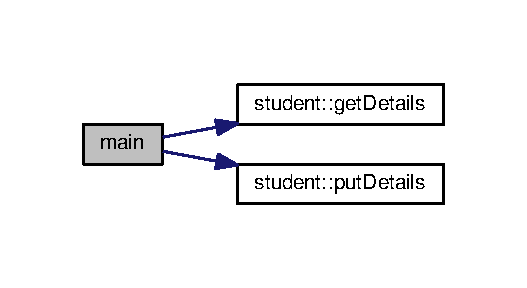
\includegraphics[width=253pt]{StudentDetails_8cpp_ae66f6b31b5ad750f1fe042a706a4e3d4_cgraph}
\end{center}
\end{figure}



%--- End generated contents ---

% Index
\backmatter
\newpage
\phantomsection
\clearemptydoublepage
\addcontentsline{toc}{chapter}{Index}
\printindex

\end{document}
